\documentclass[12pt, a4paper]{article}

\usepackage{graphicx}
\usepackage[utf8x]{inputenc}
\usepackage[croatian,english]{babel}
\usepackage[T1]{fontenc}


%\usepackage[cmintegrals,cmbraces]{newtxmath}
%\usepackage{ebgaramond-maths}
\usepackage{sectsty}
\allsectionsfont{\sffamily}
%\usepackage[scaled]{helvet}
%\renewcommand\familydefault{\sfdefault} 

\usepackage{fancyhdr}
\usepackage{times}
\usepackage{cite}
\usepackage[top=2.5cm, bottom=2.5cm, left=3cm, right=2.5cm]{geometry}

\usepackage{setspace}
\linespread{1.5}


\usepackage{secdot} % tocka za broj section, subsection
\sectiondot{subsection}
%\usepackage{enumerate}


\usepackage[toc,page]{appendix}
\usepackage{pdfpages}
% ime appendixa na hrvatskom
\addto\captionscroatian{%
   \renewcommand{\appendixtocname}{Dodaci}%
   \renewcommand{\appendixpagename}{Dodaci}%
}


\usepackage[hyphens]{url}
\usepackage{hyperref} 
%\hypersetup{pdfborder={0 0 100}}

%\usepackage{tabularx}
\usepackage{longtable}
\usepackage[labelfont={bf}]{caption}
\usepackage{verbatim}
\usepackage{subfig}




\usepackage{nonfloat}
\usepackage{parskip} %razmak izmedju paragrafa

\usepackage{indentfirst}
\setlength{\parindent}{1.5cm}


\usepackage{listings}
\lstset{
language=C,
basicstyle=\footnotesize\ttfamily,
columns=fullflexible,
showstringspaces=false
frame=single,                   % adds a frame around the code
tabsize=2,                      % sets default tabsize to 2 spaces
captionpos=b,
framexleftmargin=5mm, frame=single, frameshape={RYR}{Y}{Y}{RYR}, 
aboveskip=1cm, belowskip=0.5cm
}

\renewcommand*\lstlistingname{Ispis}
\newcommand{\headerdata}[3]{{\large\bfseries\center #1\\ \vspace*{0.2cm} #2\\ \vspace*{0.2cm} #3\par}}
\newcommand{\thesisdata}[3]{{\large\bfseries\raggedright #1\\ \vspace*{0.5cm} #2\\ \vspace*{0.5cm} #3\par}}


\usepackage{etoolbox}



\makeatletter
\AtBeginEnvironment{appendices}{%
  \clearpage%
  \fancypagestyle{plain}{%
    \fancyhf{}%
    \renewcommand{\headrulewidth}{0pt}
  }
  \thispagestyle{plain}
}






\begin{document}
\selectlanguage{croatian}
\pagenumbering{gobble} % Remove page numbers (and reset to 1)
\begin{titlepage}

%\fontfamily{cmr}\selectfont

\bfseries
\headerdata
{SVEUČILIŠTE U SPLITU}
{SVEUČILIŠNI ODJEL ZA STRUČNE STUDIJE}
{Odsjek za informacijsku tehnologiju}

\vspace*{4cm}
\begin{center}

\vspace*{3cm}

\vspace*{0.5cm}
\Huge UPUTE ZA IZRADU ZAVRŠNOG RADA NA ODSJEKU ZA IT

\end{center}
\begin{center}
\vfill
% Bottom of the page
{\large Split, \today}
\end{center}
\end{titlepage}

\clearpage
\newpage

\pagenumbering{roman}% Roman page numbers (and reset to 1)
\begin{spacing}{1.5}
\tableofcontents
\end{spacing}
\clearpage
\newpage

% za ostale stranice
\pagenumbering{arabic} % Arabic page numbers (and reset to 1)

 % numeracija i naslovnice
\section*{Sažetak}
\label{sec:summary}
\addcontentsline{toc}{section}{\nameref{sec:summary}}
Sažetak je kratki opis završnog rada. Navodi se problem, postupak rješavanja problema i cilj završnog rada. U ovom radu opisan je postupak izrade i preporuke za pisanje završnog rada. % Sam rad može poslužiti kao predložak.

\noindent\textbf{Ključne riječi}: \textit{(abecednim redom navesti najviše 5 ključnih riječi odvojenih zarezom)}

\selectlanguage{english}
\section*{Summary}
\subsection*{Title in English}
This is an example summary.

\noindent\textbf{Keywords:} ...

\newpage

\selectlanguage{croatian}
\section{Uvod}
Prilikom pisanja seminarskih i završnih radova, studenti se suočavaju sa problemom "kako pisati". Na žalost, tijekom školovanja rijetko su u prilici pisati seminarske radove pa tako nemaju dobru praksu. Veliki problem predstavlja nepostojanje materijala kojima bi ih se uputilo u osnove pravilnog pisanja radova. Namjena ovog teksta 
je obuhvatiti na jednom 
mjestu osnovne smjernice za pisanje završnog rada.

Sam postupak opisan je u Pravilniku za izradu i obranu završnih radova koji je dostupan na našim internetskim stranicama.
%Ove upute su sažetak tog pravilnika s nekim dodatnim napomenama.

%Nekoliko stvari utječe na kvalitetu rada. Prvi dojam pri čitanju dobije se na temelju izgleda dokumenta. Važno je rad korektno formatirati, odabrati fontove, veličine slova i prorede koji su ugodni za čitanje i ne odvraćaju pozornost čitatelja sa teme. Studenti su dužni pisati pravopisno i gramatički ispravne i smislene rečenice. Radove koji nisu pravopisno i gramatički ispravno napisani, mentor neće prihvatiti.

%Najvažnije pravilo kojega se studenti moraju pridržavati prilikom izrade rada je izbjegavanje plagijata. Zabranjeno je doslovno preuzimati tuđe rečenice i dijelove teksta. Ukoliko se želi citirati nekog drugog autora, potrebno je navesti izvor citata i to u obliku fusnote ili sa oznakom koja upućuje na popis literature\nocite{*}. Doslovni prijevod teksta sa nekog drugog jezika je također plagijat.

U ovom tekstu navode se osnovne smjernice za izradu završnog rada. Osim toga, ovaj dokument može poslužiti kao \LaTeX \ predložak za pisanje završnog rada. Svi izrazi koji se koriste u tekstu, a imaju rodno značenje, obuhvaćaju na jednak način sve rodove. 

U uvodu se opisuje problem koji se rješava u završnom radu, motivacija za odabir problema, kratki opis načina na koji je problem riješen te glavni doprinos rješenja s obzirom na dani problem. Na kraju uvoda daje se sažeti opis ostalih poglavlja rada. 

Nakon uvoda, u drugom poglavlju dan je postupak prijave i izrade završnog rada. U trećem 
poglavlju je opisana struktura završnog rada i dane su smjernice za oblikovanje rada. Na kraju, u zadnjem poglavlju je dan zaključak.


 
\newpage
\section{Postupak prijave i izrade završnog rada}
Završni rad na preddiplomskom studiju IT-a vrednovan je s 12 ECTS bodova što predstavlja 360 sati rada, a na specijalističkom 20 ETCS bodova (600 sati rada). %Na preddiplomskom studiju je uglavnom predviđeno da student za praktični dio rada (analiza, prikupljanje zahtjeva, teoretsko istraživanje, izrada aplikacije) iskoristi 300 sati, a za samo pisanje i pripremu obrane preostalih 60 sati. Na specijalističkom studiju IT-a rad je vrednovan s 20 ECTS bodova što predstavlja 600 sati rada, tj.~predviđeno je da student za praktični dio rada (analiza, prikupljanje zahtjeva, teoretsko istraživanje, izrada aplikacije) iskoristi približno 420 sati, a za samo pisanje i pripremu obrane preostalih 180 sati.

Priprema završnog rada započinje odabirom mentora i teme, nastavlja se izradom rada u suradnji s mentorom i završava se obranom pred povjerenstvom. Uspješno obranjen završni rad je formalni završetak školovanja na studiju čime se službeno stječu sva prava i obveze stručnog prvostupnika inženjera IT-a odnosno stručnog specijalista inženjera IT-a. 

\subsection{Odabir mentora i teme}
Izrada završnog rada je sastavni dio zadnjeg semestra studija. Da bi prijavili rad za obranu potrebno je prethodno položiti sve predmete upisane po studijskom programu i uspješno odraditi stručnu praksu.

Mentori se biraju početkom akademske godine, a studenti moraju pratiti obavijesti na kolegiju "Završni rad" na sustavu Moodle. Početkom godine Odsjek za IT objavljuje i kalendar aktivnosti, kao i dokument koji detaljno propisuje pravila za odabir mentora i recenziju radova.

Mentora se odabire obzirom na područje studija koje vas najviše zanima. Tema mora obavezno biti iz područja računalstva. S mentorom možete dogovoriti i neku temu koja još nije objavljena pazeći pritom na složenost zadatka koja mora biti u skladu s navedenim ECTS bodovima. Tema se definira barem tri mjeseca prije planirane obrane. U suradnji s mentorom jasno odredite ciljeve izrade završnog rada i ispunite obrazac za razradu teme po ECTS bodovima. Sve teme mora odobriti kolegij Odsjeka za IT prije nego se službeno odobre studentima.

U postupku odabira mentora treba uzeti u obzir da pojedini nastavnik nije obvezan prihvatiti mentorstvo, a svaki student može od pročelnika odsjeka zatražiti da mu se dodijeli mentor. Rokovi za odabir mentora propisani su Kalendarom aktivnosti.

\subsection{Izrada rada}
Preporučljivo je s izradom završnog rada započeti u zadnjem semestru studija, uz paralelno uspješno izvršavanje obaveza koje su zadane na predmetima u tom semestru.

Završni rad mora biti samostalno izrađen pod vodstvom i u suradnji s mentorom. Za sadržaj rada je odgovoran isključivo student, a mentor mu u dobroj vjeri pomaže i savjetuje ga pri samoj izradi.

Svaki pokušaj plagiranja će biti najstrože sankcioniran.

Mentor može uvjetovati obavezu korištenja nekih od alata za kolaboraciju ili verzioniranje programskog k\^oda. U tom slučaju k\^od praktičnog dijela završnog rada (a poželjno je i pismeni dio) mora biti pohranjen na nekom repozitoriju koji omogućava rad sa nekim od \textit{version control} sustava (npr. git, cvs, subversion). Mentor mora imati pristup repozitoriju. Na taj način sva povijest izrade projekta ostaje zabilježena što olakšava praćenje projekta i povratak na neku stariju/ispravnu verziju. Ukoliko pisani dio nije verzioniran putem \textit{version control} sustava, iz naziva poslanih (na čitanje) datoteka treba biti jasna njihova pozicija u vremenu.  
 
Repozitorije možete kreirati na servisima \url{github.com}, \url{bitbucket.org} ili nekom trećem. Za rad za \textit{version control} sustavom možete koristiti neki od GUI klijenata za rad sa 
 \texttt{git}-om (\url{git-scm.com/downloads/guis}), \texttt{subversion} sustavom (\url{http://svn-ref.assembla.com/windows-svn-client-reviews.html}) ili raditi iz komandne linije.
 
\subsection{Predaja rada}
Prije predaje rada student mora ispuniti sve ostale obaveze studijskog programa. Po završetku izrade rada mentor će od Pročelnika Odsjeka IT-a zatražiti formiranje Povjerenstva za završni rad. Povjerenstvo je sastavljeno od tri člana. Predsjednik povjerenstva je mentor, a uz njega su još i dva visokoškolska nastavnika. Povjerenstvo pregledava rad i ustanovljuje njegovu usklađenost s odobrenom temom te obavještava mentora o eventualnim korekcijama koje je potrebno učiniti u radu. Povjerenstvo može i odbiti rad ukoliko student nije izradio rad u skladu s temom ili je nije realizirao na zadovoljavajući način prema dogovorenim uvjetima. Postupak korekcija rada nastavlja se sve dok povjerenstvo (svi njegovi članovi) nisu prihvatili rad za predaju. 

Ukoliko je student napravio ispravke po uputama povjerenstva, mentor odobrava tiskanje dva primjerka rada na kojima će on potpisom potvrditi prikladnost za obranu. Ta dva primjerka zajedno sa CD-om na kojem se nalaze svi dokumenti i aplikacija predaju se u studentsku službu. Detalji o načinu predaje rada, obrani i ostalom određeni su Pravilnikom za izradu i obranu završnog rada koji se nalazi na \url{https://www.oss.unist.hr}) u kategoriji "Pravilnici o izradi i obrani završnog rada".

Rad se u pravilu uvezuje spiralnim uvezom. Rad može biti tiskan crno-bijelom tehnikom ako u njemu nema specifičnih detalja koji bi se izgubili takvim tiskom. Bitno je da se na CD-u nalazi i datoteka s pisanim dijelom rada koji je u skladu sa standardom PDF/A – ISO 19005 (detalji o natpisu na CD-u, nazivima datoteka i slično propisani su Pravilnikom). Uz rad se prilažu i ispunjeni obrasci (dostupni na web stranici fakulteta):

\begin{itemize}
\item Zahtjev za odobrenje teme završnog rada
\item Prijava za pristup obrani završnog rada
\item Izjava o akademskoj čestitosti
\item Izjava o pohrani završnog rada u digitalni repozitorij Sveučilišta u Splitu 
\end{itemize}

U obrascu "Prijava za pristup obrani završnog rada", stavke o znanstvenom području i polju upisuju se na sljedeći način:
\begin{itemize}
\item Znanstveno područje: Tehničke znanosti
\item Znanstveno polje: Računarstvo (u dogovoru s mentorom rad može pokrivati još neko drugo polje)
\end{itemize}

Rokovi za predaju rada propisani su Pravilnikom. Prije toga treba završiti gore opisani postupak. Kako bi bili sigurni da će rad biti predan u željenom roku trebali bi najmanje osam radnih dana prije planirane predaje imati konačnu verziju koju će mentor poslati povjerenstvu na pregled. U načelu, to bi značilo da je praktični dio rada (aplikacija) završen 20 dana prije planirane predaje. Predlažemo da se o dinamici izrade završnog rada dogovorite sa svojim vašim mentorom.

\subsection{Obrana rada}
Nakon uspješne predaje rada potrebno je obaviti i usmenu obranu rada. Student je dužan napisati prezentaciju kojom predstavlja svoj rad pred povjerenstvom. Povjerenstvo je sastavljeno od tri člana. Obrana rada je javna i vodi je predsjednik povjerenstva. Za prezentaciju se može koristiti računalo i projektor u učionici. Dodatna oprema može se koristiti u dogovoru s mentorom.

Izlaganje na obrani završnog rada treba biti kratko i koncizno, pri čemu student treba prikazati prezentaciju i praktični dio rada. Ukupno trajanje izlaganja treba biti između 15 i 20 minuta. Kao i sam rad, izlaganje treba imati strukturu: uvod, opis završnog rada, zaključak. Izlaganje počinje uvodom u materiju, gdje se opisuje tema i motivacija za temu, a završava zaključkom.

Izlaganje treba biti fluidno. Treba izbjegavati čitanje pripremljenog materijala. U tu svrhu dobra je preporuka nekoliko puta kući isprobati izlaganje. Pristupnik prezentira završni rad u stojećem položaju, okrenut prema povjerenstvu (a ne prema ploči).

Nakon izlaganja članovi povjerenstva postavljaju pitanja studentu, te se eventualno traži prezentacija praktičnog dijela. 

Nakon obrane student izlazi iz učionice, a povjerenstvo održi kratki sastanak na kojem se ocjenjuje rad i obrana. Pri povratku predsjednik povjerenstva objavljuje ocjene za rad, obranu te konačnu ocjenu završnog rada. 

Službena potvrda o završetku studija i stečenom nazivu može se predignuti u studentskoj referadi u pravilu sedam dana nakon obrane.
\newpage
\section{Oblikovanje završnog rada}

\subsection{Odabir uređivača teksta}

Za pisanje rada možete koristiti bilo koji program za obradu teksta (engl.~\textit{word processor}) kao što su Microsoft Office, LibreOffice i Google Documents ili slovoslagarski program npr.~\LaTeX. Bez obzira koji se alati za oblikovanje teksta koriste, završni rad mora biti korektno formatiran. U slučaju da se koristi neki od WYSWYG (\textit{what you see is what you get}) uređivača teksta preporuka je da se unaprijed definira 
stil dokumenta. Dakle, unaprijed se definiraju veličine naslova, podnaslova, fontovi i slično. Važno je da određeni stil prati cijeli završni rad. 


U slučaju da student želi koristiti \LaTeX, može dobiti predložak ovog dokumenta za pomoć pri izradi rada.

\subsection{Osnovne postavke oblikovanja teksta}
Prilikom izrade tekstualnog dijela završnog rada treba pratiti sljedeće upute:
\begin{itemize}
 \item Format papira A4.
 \item Font Times New Roman ili neki slični, veličina 12pt.
 \item Margine:
 \begin{itemize}
  \item gornji rub: 25 mm
  \item donji rub: 30 mm
  \item unutarnji rub (lijevi): 30 mm
  \item vanjski rub (desni): 25 mm
 \end{itemize}
 \item Obostrano poravnanje.
 \item Prored teksta 1.5 (engl.~\textit{line spacing}).
 \item Početak odlomka mora biti uvučen. Redak se uvlači na početku svakog odlomka. Između odlomaka treba biti veći razmak.
 
 \end{itemize}
%\subsubsection*{Numeriranje}
Naslovnica nije numerirana. Sadržaj je numeriran rimskim brojevima. Sve ostale stranice u završnom radu trebaju biti numerirane arapskim brojevima unutar donje margine. 

\subsection{Struktura završnog rada}
\textbf{Naslovna} i \textbf{prva stranica} završnog rada definirane su Pravilnikom za izradu i obranu završnog rada. Njih slijedi \textbf{sadržaj} koji treba biti generiran iz naslova poglavlja i potpoglavlja.

Slijedi \textbf{sažetak} u kojem u nekoliko rečenica treba navesti što je cilj završnog rada i kako se do njega došlo (što je analizirano, razvijeno, izrađeno). Na kraju sažetka mogu se navesti ključne riječi koje su važne za rad. Na istoj stranici ispod sažetka treba napisati i sažetak na engleskom jeziku (engl.~\textit{summary}). Na početku sažetka na engleskom jeziku treba podebljanim tekstom napisati naziv teme na engleskom jeziku. Kao i za sažetak na hrvatskom treba prevesti ključne riječi na engleski jezik (engl.~\textit{keywords}).

Potom se u \textbf{uvodu} opisuje problem, motivacija za rad (zbog čega je ponuđeno rješenje uopće potrebno) i način na koji ste rješavali problem te glavni doprinosi. Na kraju uvoda sažeto se opisuju ostala poglavlja rada.

\textbf{Glavni dio} treba suvislo podijeliti na više poglavlja. U pravilu se počne sa specifikacijom te poglavljem o metodama i alatima koji su korišteni (opis metoda, opis alata, primjeri tipične uporabe i sl.). U idućem poglavlju opisuje se sam rad i doprinosi. Na primjer, detaljno se opisuje metoda ili sustav koji je razvijen prilikom izrade završnog rada te detaljan opis implementacije. Ako se razvijaju samo dijelovi sustava, tj.~neke komponente sustava, mogu se dati primjeri upotrebe. U sljedećem poglavlju može se detaljno opisati aplikaciju odnosno praktični rad. Ako sustav ima korisničko sučelje slikama se prikazuju snimke zaslona pri tipičnoj uporabi aplikacije. Ako se u radu razvija novu metodu, ovo poglavlje može biti namijenjeno njenoj eksperimentalnoj evaluaciji i raspravi o eksperimentalnim rezultatima.

Na kraju se piše \textbf{zaključak}. On može početi s jednostavnim opisom što je u radu napravljeno i koji su glavni doprinosi rada. Nakon toga može se napisati nekoliko rečenica u kojima se opisuje zašto je napravljeno uopće važno, kakva je moguća upotreba i što se predlože kako bi se napravljeno poboljšalo u skladu s postavljenim ciljevima. Ako se razvijena aplikacija već koristi mogu se opisati povratne informacije korisnika.

U \textbf{literaturi} se navode izvori po redoslijedu pojavljivanja u tekstu. Navode se samo oni izvore na koje se u radu poziva.

Na kraju rada treba dodati i \textbf{izjava o autentičnosti završnog rada} koja se nalazi na našim internetskim stranicama.

\subsection{Slike, tablice i programski k\^od}
U završni rad uključuju se slikovni prikazi (grafovi, sheme, ilustracije, snimke zaslona i sl.) koji povećavaju razumljivost i čitljivost rada. Slike moraju biti numerirane u tekstu te imati odgovarajući naziv (engl.~\textit{caption}) neposredno ispod slike. U rad umetnite slike otprilike uz dio teksta iz kojeg se pozivate na njih. Svaka slika treba biti referirana na barem jednom mjestu u tekstu. Slike centrirajte kao i njihov naziv. Primjerice, na slici~\ref{fig:xfce} je prikazan jedan od bezbroj mogućih izgleda radne okoline.
\\[\intextsep]
\begin{minipage}{\linewidth}
\centering%
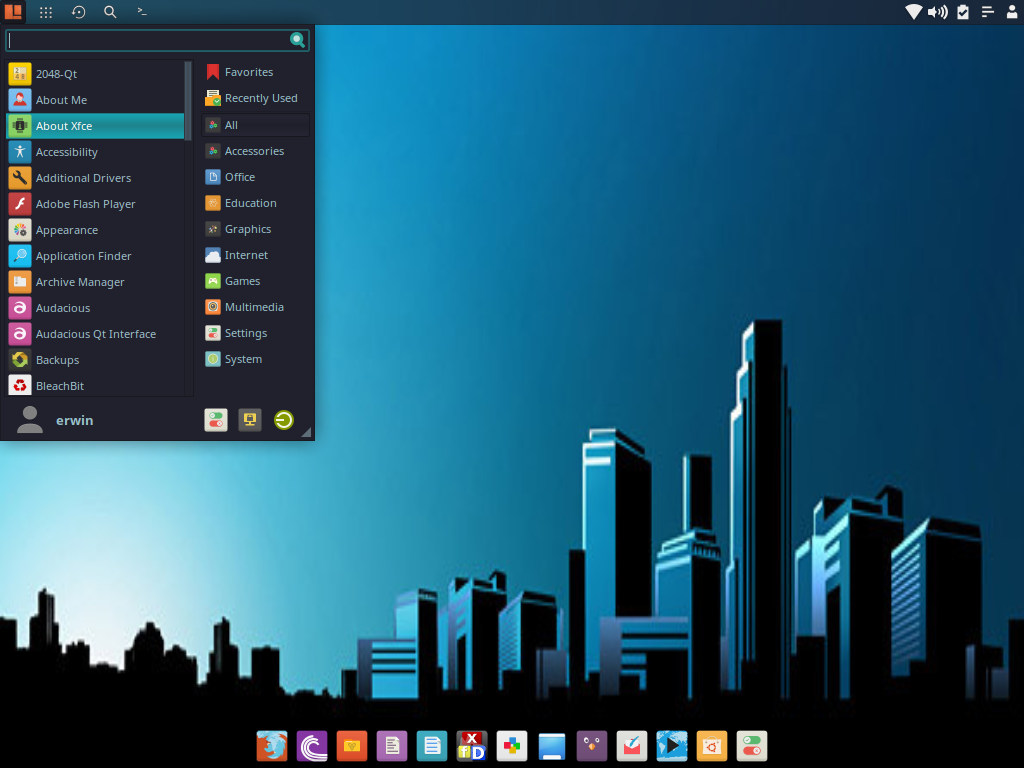
\includegraphics[width=0.4\linewidth,clip=]{slike/xfce.png}
\figcaption{Primjer radne okoline Xfce}%
\label{fig:xfce}%
\end{minipage}
\\[\intextsep]
Rezultati eksperimenata mogu se prikazati u tablicama koje moraju biti numerirane i imati naziv kao i slike. Naziv i opis tablice nalazi se neposredno iznad tablice. Tablica mora biti referirana na barem jednom mjestu u tekstu, kao u sljedećem primjeru: U tablici~\ref{fig:ioesc} opisane su najčešće \textit{escape} sekvence.
\begin{longtable}{l l }
\caption{Escape sekvence}\label{fig:ioesc}
\endfirsthead
\endhead
\hline
oznaka&opis \\
\hline
\lstinline!\n!&novi red \\
\lstinline!\t!&horizontalni tab\\
\lstinline!\v!&vertikalni tab\\
\lstinline!\'!&apostrof \\
\lstinline!\"!&dvostruki navodnik \\
\lstinline!\\!&\textit{backslash} znak \\
\lstinline!\?!&upitnik\\
\hline
\end{longtable}

Programski k\^od se piše fontom u kojem su sva slova jednake širine (engl.~\textit{monospace}). Primjer takvog fonta je \texttt{courier}. %Listu slobodnih \textit{monospace} fontova možete naći na stranicama \url{http://www.fontsquirrel.com/fonts/list/classification/monospaced}. 
Veličina slova treba biti nešto manja nego u običnom tekstu. Primjer k\^oda je dan u ispisu~\ref{program}.
%
%\begin{lstlisting}
%#! /bin/bash
%# skripta za prebacivanje "layout-a" tipkovnice
%setxkbmap $1
%echo Prebacili ste na $1 tipkovnicu.
%\end{lstlisting}
%\caption{Skripta za mijenjanje položaja tipkovnice}
%\label{fig:program}
%\end{figure}

\begin{lstlisting}[caption={Skripta za mijenjanje rasporeda tipki tipkovnice}, label=program]
#! /bin/bash
# skripta za mijenjanje "layout-a" tipkovnice
setxkbmap $1
echo Prebacili ste na $1 tipkovnicu.
\end{lstlisting}

U tekstu prilikom navođenja naziva varijabli, memorijskih lokacija, putanja i naziva direktorija i datoteka, naziva metoda i funkcija koristi se neki iz \texttt{monospace} obitelji fontova.
\subsection{Pravopis i gramatika}

Studenti su obavezni predati pravopisno i gramatički ispravan rad. Završni radovi koji nisu ispravno napisani neće biti mentorirani. Provjera ispravnosti riječi može se obaviti putem stranice \href{http://hjp.znanje.hr/}{hrvatskog jezičnog portala}. Pravila hrvatskog pravopisa mogu se naći na stranicama \href{www.pravopis.hr}{www.pravopis.hr}. Među pravilima treba obratiti pažnju na pisanje tuđica, koje su uobičajene u pisanju radova iz područja računarstva. Osim toga, obavezna je i provjera teksta alatima za jezičnu provjeru (engl.~\textit{spell checker}) hrvatskog jezika. Ako ga nemate, na stranicama \url{https://hacheck.tel.fer.hr/} nalazi se online alat.
\subsection{Kratice}

Prilikom prvog pojavljivanja, kratice u tekstu se opisuju, a u daljnjem tekstu se koriste bez ponovnog opisa. 

\subsection{Strane riječi}
U završnom radu koristi se hrvatski jezik kada za određenu riječ postoji hrvatski prijevod. Ukoliko korištenje takve hrvatske riječi nije 
uobičajeno u praksi ili autori rada ne 
poznaju odgovarajuću hrvatsku riječ, ostavlja se strana riječ napisana \textit{u kurzivu}.

Kada se prvi put uvodi pojam na hrvatskom jeziku, potrebno je u zagradama navesti i originalnu riječ. Npr. jezgra (engl.~\textit{kernel}) operativnog sustava.  

\subsection{Stil}
Završni rad se piše u neutralnom stilu i bezlično npr. "ispitivanje je pokazalo...". 
Preporučljivo je izbjegavati prvo lice jednine i prvo lice množine osim na mjestima gdje se ističe osobna odluka između više mogućnosti. 


\subsection{Popis literature}
Navode koji su preuzeti iz vanjskih izvora potrebno je potkrijepiti referencom (broj u uglatim zagradama po redoslijedu pojavljivanja). Broj se odnosi na izvor podataka naveden u popisu literature. Fusnote na dnu stranice treba izbjegavati jer nisu uobičajeni oblik citiranja za tehničke radove. Internetski izvori moraju imati u zagradama na kraju datum kad je stranica zadnji put posjećena. Reference treba oblikovati prema IEEE stilu pisanja radova~\cite{IEEE}.

U popisu literature treba navesti literaturu koja se koristila za izradu rada te popis web stranica. Izvore navedite po redoslijedu pojavljivanja u tekstu. Navedite samo one izvore na koje se u radu pozivate. Popisi trebaju biti 
grupirani na način da se najprije navede popis literature, a zatim popis web stranica s datumom zadnjeg pristupanja stranici. Literatura se navodi kako slijedi:
\begin{enumerate}
\item 
Prezime autora, inicijal imena: Naslov knjige, izdavač, mjesto i godina izdavanja
\item Prezime autora, inicijal imena: Naslov rada, naziv skupa, časopisa ili zbornika radova,
mjesto i godina objavljivanja
\item Prezime autora, inicijal imena: Naslov rada, web stranica objavljivanja
\end{enumerate}

\subsection{Plagiranje}

Citiranje je doslovno preuzimanje dijelova drugog rada. Citira se u navodnicima uz referencu na izvor podataka. 
Svako preuzimanje dijelova teksta koji nije ispravno citiran smatra se plagijatom i nije dopušteno u izradi završnog rada.

Parafraziranje je vlastitim riječima opisan dio drugog rada, u kojem slučaju je potrebno navesti izvor 
parafraziranog teksta. Doslovno prevođenje sa stranog jezika smatra se plagijatom. Ukoliko student pošalje rad za koji mentor utvrdi da je plagiran u bilo kojem dijelu teksta, mentor neće mentorirati ni ispravljati ostatak završnog rada.

\subsection{Imenovanje dokumenta}
Završni rad predaje se u pdf formatu. Ukoliko se tijekom izrade šalje na provjeru mentoru, svaka nova verzija dokumenta treba biti 
ispravno numerirana kako bi se iz imena 
dokumenta lako moglo odrediti da li je dokument noviji od prethodno poslanih. Npr.~pet dokumenata koji se šalju na čitanje mogu biti 
imenovani na sljedeći način:
\\
\texttt{prezime\_zavrsni\_1.0.pdf}\\
\texttt{prezime\_zavrsni\_1.1.pdf}\\
\texttt{prezime\_zavrsni\_1.2.pdf}\\
\texttt{prezime\_zavrsni\_1.3.pdf}\\
\texttt{prezime\_zavrsni\_2.0.pdf}\\
Nula na kraju imena (1.0, 2.0 itd) označava verzije sa važnim izmjenama, dok se verzije sa manjim izmjenama označavaju ostalim brojevima (1.1, 1.2, 2.1 itd). 

Osim navedene mogućnosti numeriranja, postoji mogućnost da pri izradi završni rada koristi neki do sustava za kontrolu verzija (\textit{git, subversion, cvs}). Odabir takve mogućnosti je poželjan.

\subsection{Jezični savjeti}
\begin{itemize}
\item 
Završni rad je napisan na hrvatskom jeziku. Možda će uskoro biti moguće pisati i na nekom od svjetskih jezika, ali za sada je moguće jedino na hrvatskom jeziku.
\item Završni rad mora biti napisan u skladu sa standardom i pravilima jezika. Preporučujemo da pismeni dio rada pregleda lektor ili ga pregledajte na neki drugi način. Stručni rad nije literalni tekst pa za njega vrijede drukčija pravila.
\item Stručni tekst mora biti jednoznačan, stoga pišite u kratkim, jednostavnim i jasnim rečenicama.
\item Pišite u neutralnom stilu u pasivu, npr.: „razvijen je“, „napravljeno je“, „napisano je“ i sl. Izbjegavajte prvo lice jednine i množine osim na mjestima na kojima želite istaknuti svoju osobnu odluku između više mogućnosti. 
\item Za pojedini pojam ili objekt u cijelom radu koristite istu oznaku ili ime.
\item Ako uvodite nove pojmove pazite da su jednoznačno i pravilno definirani.
\item Koristite važeću stručnu terminologiju (ne server nego poslužitelj, ne hardware nego strojna oprema ili eventualno hardver, ne elektronska pošta nego elektronička pošta, ne računar nego računalo, ne router ili ruter nego usmjernik, ne Internet nego internet). Postoji mnogo internetskih izvora na koja vas može uputiti vaš mentor.
S pisanjem stručnih riječi se razvija i hrvatska stručna terminologija. Tamo gdje je smisleno u suradnji s mentorom predložite hrvatski prijevod za stručne izraze koji još nemaju prijevoda.
Posebnu pozornost posvetite prijevodima s engleskog jezika. Pri tomu pazite na pravila hrvatskog jezika. Samostalni pridjevi su na hrvatskom jeziku na desnoj strani imenice ili predmeta (SQL query je upit SQL, x-axis je os x, Laravel framework je razvojni okvir Laravel, Linux operation system je operativni sustav Linux i sl.). Obratni redoslijed je pogrešan: SQL upit, x os, Laravel razvojni okvir ili Linux operativni sustav.

\item Iza znaka interpunkcije (točka, zarez, upitnik, uskličnik i slično) stavlja se razmak. Razmak dolazi i prije otvorene zagrade, ali ne i nakon otvorene zagrade i prije zatvaranja zagrade. 
Nakon zagrade ponovo se stavlja razmak.

\item Između broja i znaka za mjernu jedinicu piše se razmak.

\item Riječ k\^od piše se s akcentom.                               
\end{itemize}

\newpage

%\newpage
\section{Zaključak}
U ovom tekstu dan je pregled izrade završnog rada. Na temelju iznesenog, studenti bi trebali izraditi korektno sastavljeni završni rad. 
Naravno, najteži dio izrade je 
sadržaj rada, koji studenti moraju sami osmisliti. 
Ovaj tekst pomoći će im da izbjegnu zamke plagiranja i da uoče vrijednost samostalnog i autorskog rada.
\newpage
%\SuspendCounters{page}
%\renewcommand{\thepage}{}

\addcontentsline{toc}{section}{Literatura}
\bibliography{Zavrsni_literatura}
\bibliographystyle{IEEEtran}

\newpage
\clearpage
\phantomsection
%\renewcommand\bibname{Literatura}

\begin{appendices}
\appendix
\thispagestyle{empty}

\includepdf[pages={1-4}]{Naslovne_IT.pdf}
\end{appendices}

\end{document}
